\documentclass{standalone}
\usepackage[T1]{fontenc}
\usepackage[utf8]{inputenc}
\usepackage{pgf,tikz}
\usepackage{setspace}
\usepackage{pgfplots}
\pgfplotsset{compat=1.13}
\usepackage{romannum}

\usepgfplotslibrary{groupplots}

\begin{document}


\def\TT{1.0}

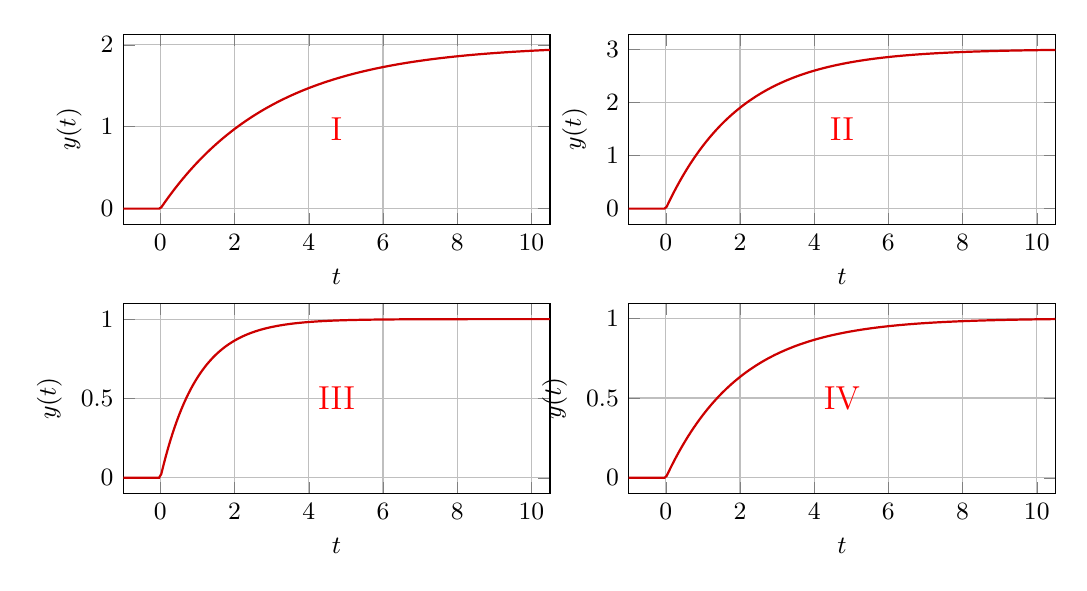
\begin{tikzpicture}
\begin{groupplot}[
  group style={group size=2 by 2},height=4cm,width=7cm,
  /tikz/font=\small,
  %xtick=0,
  %ytick=\empty,
  xlabel={$t$}, 
  ylabel={$y(t)$},
  xmin=-1,
  xmax=10.5,
  grid = both,
  ]

  \nextgroupplot
    \addplot+[thick, red!80!black, no marks, domain=-1:11, samples=200] {(x>0)*2*(1-exp(-x/3))};
    % \addplot+ 
    %shell[thick,black, no marks, prefix=pgfshell_, id=firststep,] {julia -q --eval  "using ControlSystems; H=tf([1],[1, 1, 1]); print_step(H, 10);"};

  \nextgroupplot
    \addplot+[thick, red!80!black, no marks, domain=-1:11, samples=200] {(x>0)*3*(1-exp(-x/2))};

    \nextgroupplot
    \addplot+[thick, red!80!black, no marks, domain=-1:11, samples=200] {(x>0)*(1-exp(-x/1))};

  \nextgroupplot
    \addplot+[thick, red!80!black, no marks, domain=-1:11, samples=200] {(x>0)*(1-exp(-x/2))};
  \end{groupplot}

  \node[red] at (group c1r1.center) {\large \Romannum{1}};
  \node[red] at (group c2r1.center) {\large \Romannum{2}};
  \node[red] at (group c1r2.center) {\large \Romannum{3}};
  \node[red] at (group c2r2.center) {\large \Romannum{4}};

\end{tikzpicture}
\end{document}

